\section{Experimental Pipeline}
\label{sec:methods/section_c}

Once we selected the parameters for YOLOv3 and SORT, we are ready to run the experiment for taking measurements. Figure \ref{fig:experiment_pipeline} shows the pipeline for the experiment.
\begin{figure}[!htb]
  \centering
  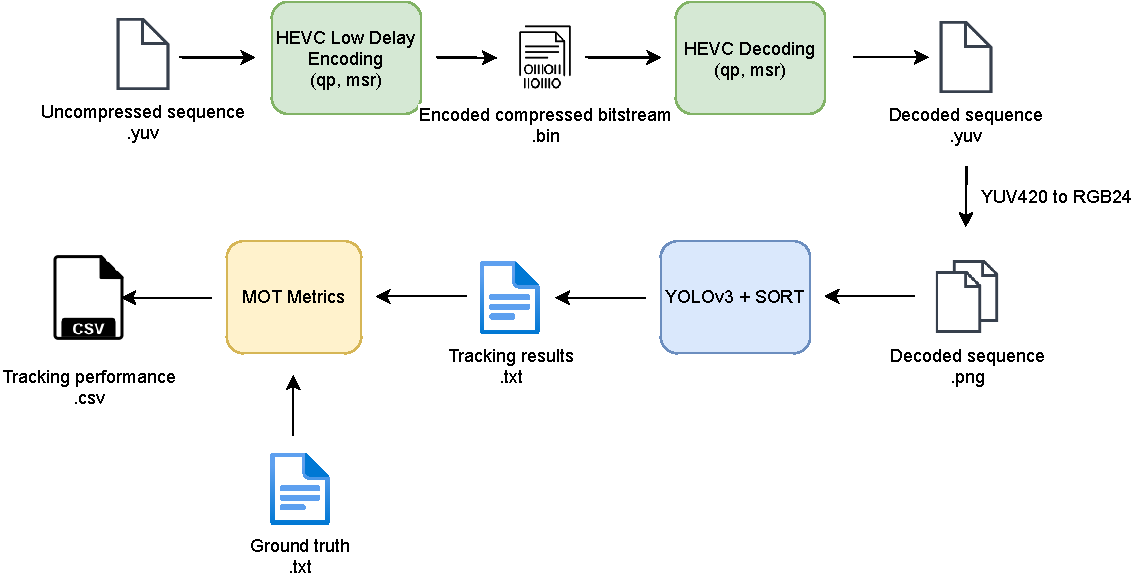
\includegraphics[width=1.0\linewidth]{img/experiment_pipeline.pdf}
  \caption[Pipeline for the experiment]
  {Pipeline for the experiment.}
  \label{fig:experiment_pipeline}
\end{figure}

The uncompressed sequences from Table \ref{tab:seq_list} were used but we excluded the training sequence of Class C PartyScene since we have used this sequence to tune the parameters to optimize the detector and tracker. Therefore, there are totally 12 sequences that were used for the analysis. HEVC video compression has been applied with different quantization parameter (QP) and motion search range (MSR). The following range of QP and MSR have been attempted for the experiment,

% \begin{myfont}
% \centering
% QP = [18, 22, 26, 30, 34, 38, 42, 46], MSR = [8, 16, 32, 64]
% \end{myfont}

\begin{table}[]
    \centering
    \begin{tabular}{|c|c|}
        \hline
        HEVC parameter & Range of values \\
        \hline
        \hline
        QP & [18, 22, 26, 30, 34, 38, 42, 46] \\
        \hline
        MSR & [8, 16, 32, 64] \\
        \hline
    \end{tabular}
    \caption{Caption}
    \label{tab:qp_msr_range}
\end{table}

\noindent The pipeline for the experiment can be broken down as following.
\begin{enumerate}
    \item \textbf{HEVC Encoding}: The experiment starts with applying HEVC encoding to the uncompressed sequences and generating the compressed bitstreams. Low Delay Encoding is used for encoding. Encoding is the process that took the most amount of time in the entire pipeline, so we encoded all the possible combination of QP and MSR and saved all the compressed bitstreams before applying decoding.
    \item \textbf{HEVC Decoding}: After obtaining all the compressed bitstreams, we apply HEVC decoding to the bitstreams and output the decoded sequences in YUV420 format.
    \item \textbf{YUV420 to RGB color conversion}: Since the YOLOv3 object detector accepts in RGB format, we convert the decoded sequences in YUV420 to RGB format in .png files.
\end{enumerate}

